\documentclass[12pt]{article}

\usepackage[a4paper, margin=1in]{geometry}
\usepackage[english]{babel}
\usepackage[utf8]{inputenc}

\usepackage[colorlinks=true, allcolors=blue]{hyperref}

\title{CRPL: Interim Report}
\author{Harrison Beau Barker}

\usepackage{graphicx}
\graphicspath{ {images/} }

\usepackage{xcolor}

\usepackage{tabularx}
\newcolumntype{b}{X}
\newcolumntype{s}{>{\hsize=.5\hsize}X}

\newcommand{\keyword}[1]{\textbf{\textit{#1}}}
\newcommand{\q}[2]{\begin{quote} #1 \cite{#2} \end{quote}}

\setlength{\parskip}{1em}
%\setlength{\parindent}{0em}
\begin{document}

\begin{titlepage}
	\centering
	
\includegraphics[width=0.4\textwidth]{crpl}\par
	\vspace{1cm}
	{\huge\bfseries CRPL: Report\par}
	\vspace{2cm}
	{\Large\itshape Harrison Beau Barker\par}
	\vfill
	{\url{https://github.com/MrHarrisonBarker/crpl}\par}
	\vspace{1cm}
	{\large Hbark002, 33575210\par}
\end{titlepage}

\abstract{TODO}

\tableofcontents{}

\section{Keywords}

\begin{description}
	\item[Copyright]
	\item[Blockchain]
	\item[Ethereum]
	\item[Smart Contract]
	\item[Open-source] 
\end{description}

\section{Introduction}

The aim of this project is to represent a version of \keyword{copyright} for protection of intellectual property on a \keyword{blockchain} backed by a public ledger of transactions. My initial impetus for this project was a book I read in 2018 called \textit{"Blockchain Revolution: How the Technology Behind Bitcoin Is Changing Money, Business, and the World"}\cite{blockchain_revolution}, before this point I knew little of the applications for blockchain technologies attributing them only to a new form of digital currency allowing peer to peer transactions of wealth.

However, this book introduced the concept of \keyword{smart contracts} and the possibilities now small immutable programs could be saved and run on a blockchain. The most relevant change smart contracts brought was progressive state into an infamously immutable technology, by leveraging an unmodifiable chain of transactions state became not just a current record (like most traditional systems) but a historical account of all previous states with a clear a definable list of transformations precisely timestamped.

This new knowledge of \keyword{blockchains} came to fruition when it came to selecting my final project but to what problem should I help to provide a solution to leveraging this technology. A combination of recent interest in the crypto-sphere mainly coming from NFTs, continued displays of a \keyword{copyright} system not fit for purpose\cite{DMCA-abuse} and the book I had read 3 years earlier proposing that \keyword{blockchain} and \keyword{smart contracts} were an extremely viable solution to problems intersecting law and social structures.

\subsection{Unfit for purpose}

So why is the current \keyword{copyright} system not fit for purpose? I've broken it into three interlinking factors; complexity, jurisdiction dependence and lack of digital computerised systems. starting with complexity, it is often hard as a creator to know if your work is protected or if the protection is enough? This gives massive power to publishers, managers and companies who are willing to exploit this fact by blinding a creative with a large contract covered in legal jargon. Should an artist also have to be a lawyer?

Jurisdiction dependence can be looked at as a point of complexity and inefficiency in the system, yes there's international \keyword{copyright} law in the form of the \textit{"Berne Convention"}\cite{Berne} and later \textit{"WIPO Copyright Treaty"}\cite{WIPO} which informs most of our modern \keyword{copyright} law. However, these treaties only state minimum requirements and standards to follow but do not control the internal \keyword{copyright} law of a sovereign nation which will always take precedence.

This idea of global \keyword{copyright} links nicely into my last factor which is centred around the digital and ever more interconnected world we're living in. Even though in 1996 the \textbf{WCT}\cite{WIPO} was introduced to address issues caused by the emergence of information technology, however the world and more specifically the internet has changed an unimaginable amount since 1996 but \keyword{copyright} is effectively unchanged including the systems to register and view registered \keyword{copyrights} which are closed off in obscurity.

\subsection{What a solution needs}

I've defined what I believe as to be four requirements of a solution to this problem and how I've addressed these requirements.

% TODO not sure about this section
\begin{description}
	\item[Global] Both the system needed to be globally accessible, available and consistent across all jurisdictions to minimise complexity and maximise protection for an interconnected world. I've implemented this by using the \keyword{Ethereum} network which is made up of thousands of nodes across the world.
	\item[Open] Openness is essential to instil trust in a completely independent and alternative solution compared with government institutions that have implied trust and guaranty. I've implemented this by writing and using \keyword{open-source} code including \keyword{Ethereum} which is \keyword{open-source} and backed by a public ledger.
	\item[Robust] The current written laws and contracts maybe complex but are strongly defined with a commonly accepted interpretation, this will have to be true in this solution. I've implemented this by using an immutable \keyword{smart contract} for copyright representation and logic.
	\item[Simple] This is the most important requirement as the proposed problem is centred around current \keyword{copyright} complexity so any solution will need to be accessible to every possible user. I've implemented this by using clearly defined selectable \keyword{copyright} protections when registering a work.
\end{description}

\section{Research}
\subsection{Blockchain}
% TODO Technical knowledge needed to implement
% TODO How it works?
% TODO Why use it?

\subsection{Existing solutions}

\subsubsection{Copyright law}
% TODO The state of the current copyright system
\subsubsection{Online rights management}
% TODO How do creators manage protection of their work

\subsection{Development theory}
% TODO Explanation of agile development methodology
% TODO TDD and Scrum

\subsection{Aims of the solution}
% TODO The over arcing aims of the solution, aka what should the system fix

\section{Design}

\subsection{Technical Requirements}
% TODO a more comprehensive and detailed list of requirements

\begin{description}
	\item[Copyright smart contract] Immutable code on a public ledger “blockchain“ for the purpose of establishing ownership or the copyright to a piece of work.
	\item[Multi-party distribution] The ability to establish a complex ownership structure which includes multiple individuals/groups.
	\item[Ownership transfer] The ability to change the ownership of a copyright from one complex structure to another with consent of all current owner(s).
	\item[Work verification] Verification of a work to establish its originality with a reasonable accuracy for the platform.
	\item[Dispute filing] Allow any user to dispute a copyright with sufficient evidence and provide an option for resolving these disputes by the owner(s).
	\item[Digital signing] Digital signing a work for authentic verification based on our records.
	\item[\color{orange}{Decentralised Work CDN & proxy}] Providing an access point for stored work within the chain.
	\item[\color{orange}{Web-socket updates}] Real-time updates for the front-end UI to provide a better end-user experience.
\end{description}

\subsection{Smart contract}
% TODO Ownership structure
% TODO Permission based protections
% TODO Inspiration from nft contract (starting point) https://eips.ethereum.org/EIPS/eip-721
% TODO Shareholder consensus mechanism

\subsection{Back-end}
% TODO Service and dependancy injection based architecture
% TODO Background service pattern
% TODO event processing patterns
% TODO state diagrams (how the flow of applications)

\subsection{Database}
% TODO what is duplicated between the chain and the database
% TODO what is only on the database and not on the chain
% TODO Express the need for synchronisation

\subsection{Front-end}
% TODO Visual design philosophy
% TODO How the use will login?
% TODO form design and working

\subsection{Development process}
% TODO how the development was laid out and planned
% TODO sprint structure

\section{Implementation}

\subsection{Smart contract}
% TODO saved metadata

\subsubsection{Interface overview}
% TODO events
% TODO ownership
% TODO copyright

\subsubsection{Registration}
% TODO Registration of copyright
% TODO how each copyright is saved (maximum size?)
% TODO approve the message sender
% TODO record all shareholders

\subsubsection{Ownership restructure}
% TODO Restructure proposal
% TODO Binding vote
% TODO Restructure event
% TODO failed restructure

\subsubsection{Modifiers}
% TODO isShareholder or approved
% TODO valid addresses
% TODO expired

\subsection{Back-end}
% TODO Service -> Controller
% TODO digital signing
% TODO ContractRepository

\subsubsection{Queries}
% TODO structured query
% TODO chain injection
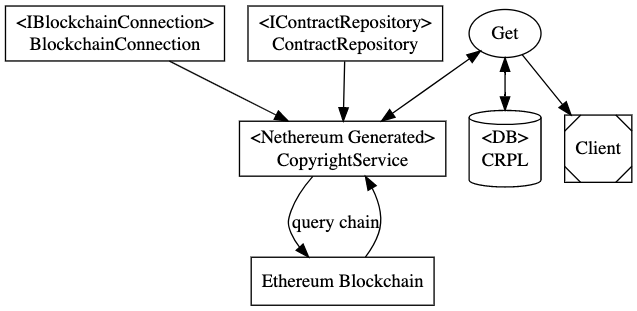
\includegraphics[width=\textwidth,height=\textheight,keepaspectratio]{images/operational/chain-inject}

\subsubsection{Registration process}
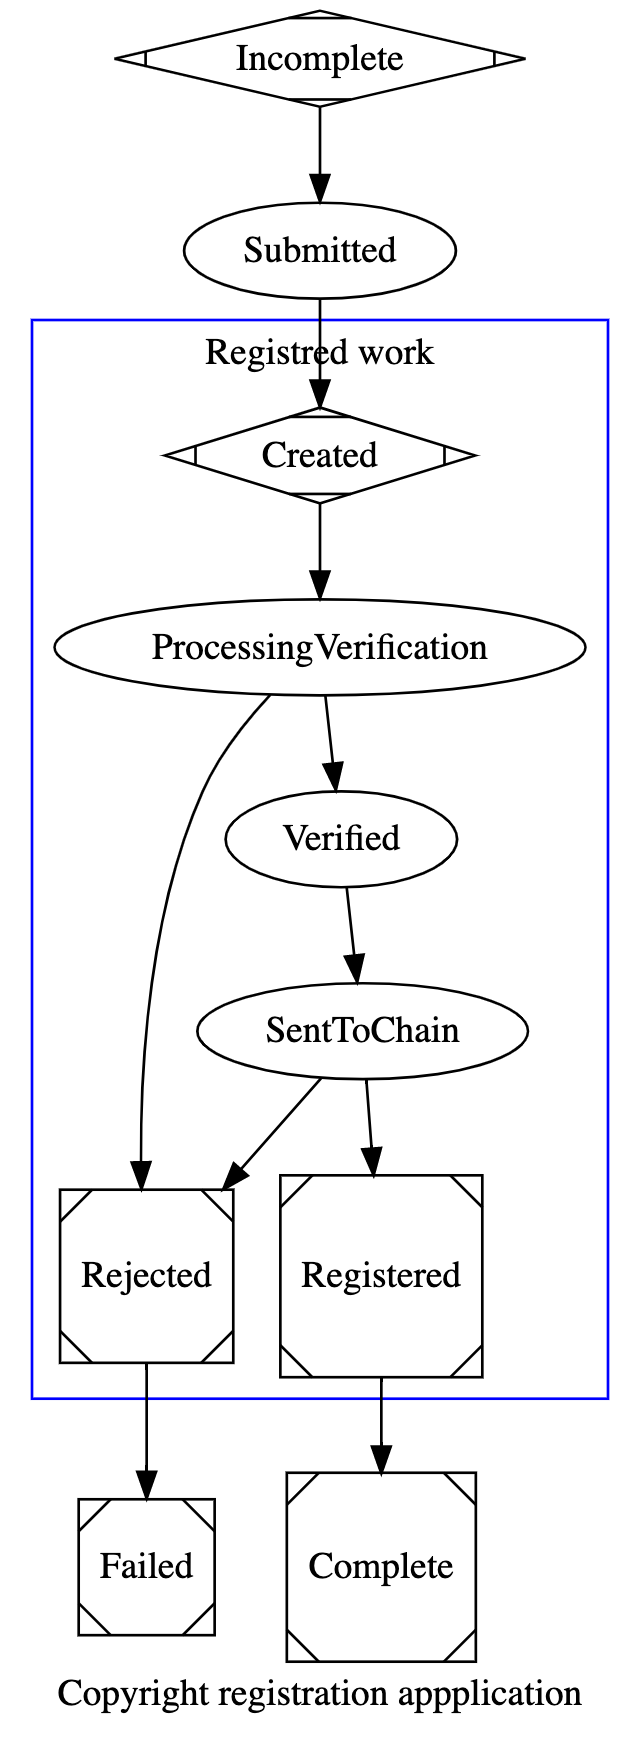
\includegraphics[width=\textwidth,height=\textheight,keepaspectratio]{images/operational/cpy-registration-status-graph}

\subsubsection{Dispute handling}
% TODO filing disputes
% TODO resolving disputes: payment, change of ownership
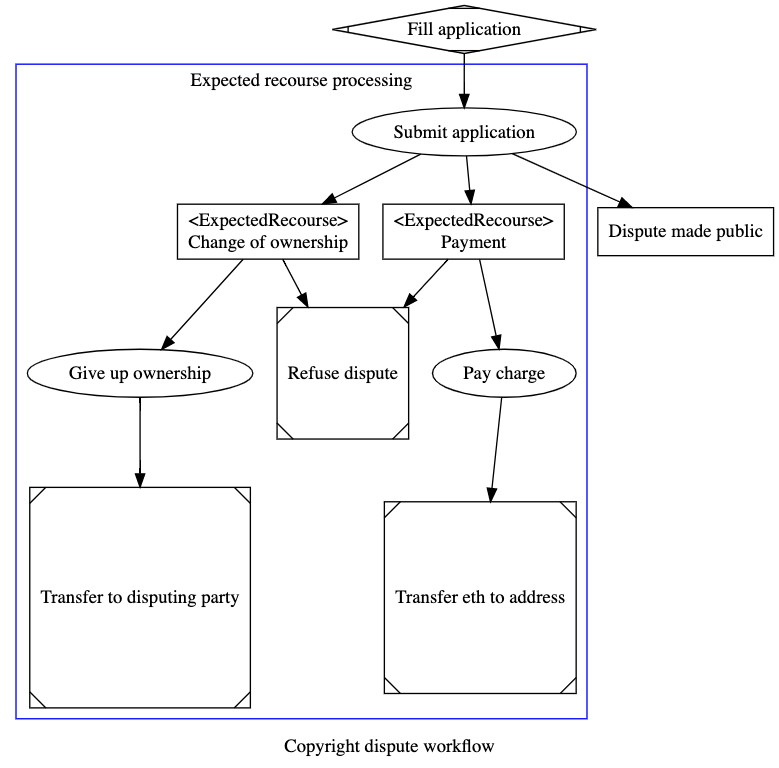
\includegraphics[width=\textwidth,height=\textheight,keepaspectratio]{images/operational/dispute-workflow}

\subsubsection{Applications framework}
% TODO Data model structure (application, view model, input model)
% TODO unified status and processing flow (update -> submit = complete)

\subsubsection{API overview}
% TODO API diagrams and structure
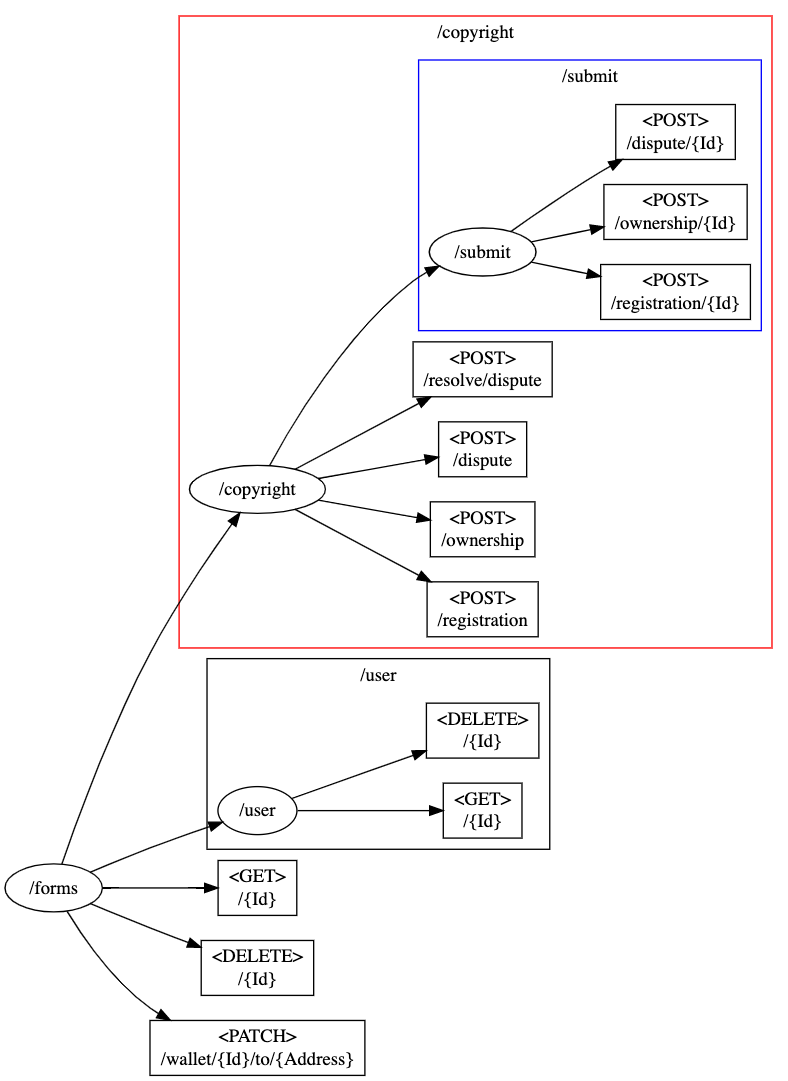
\includegraphics[width=\textwidth,height=\textheight,keepaspectratio]{images/operational/Forms-Api}

\subsubsection{Blockchain event listeners}
% TODO Blockchain event listeners
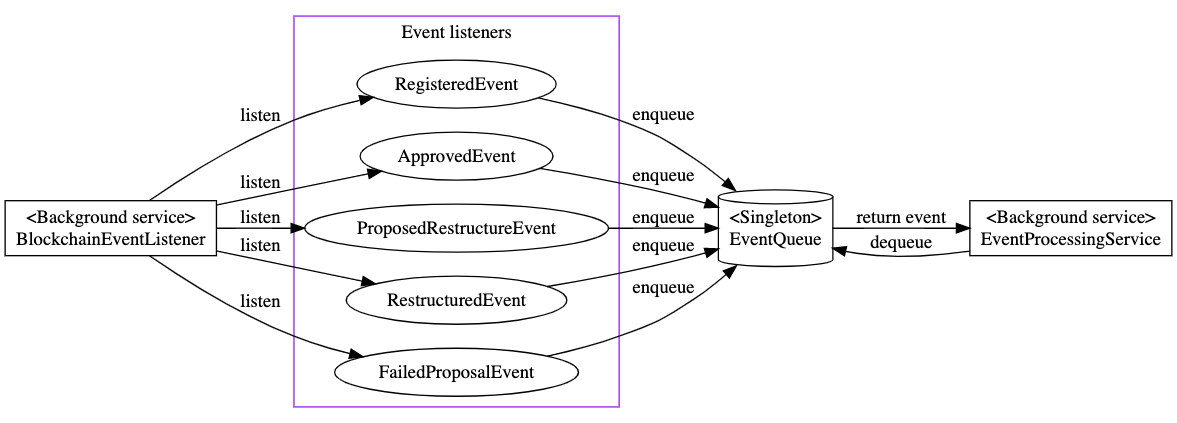
\includegraphics[width=\textwidth,height=\textheight,keepaspectratio]{images/operational/Event-Listening}


\subsubsection{Background services}
% TODO verification pipeline
% TODO Expiry

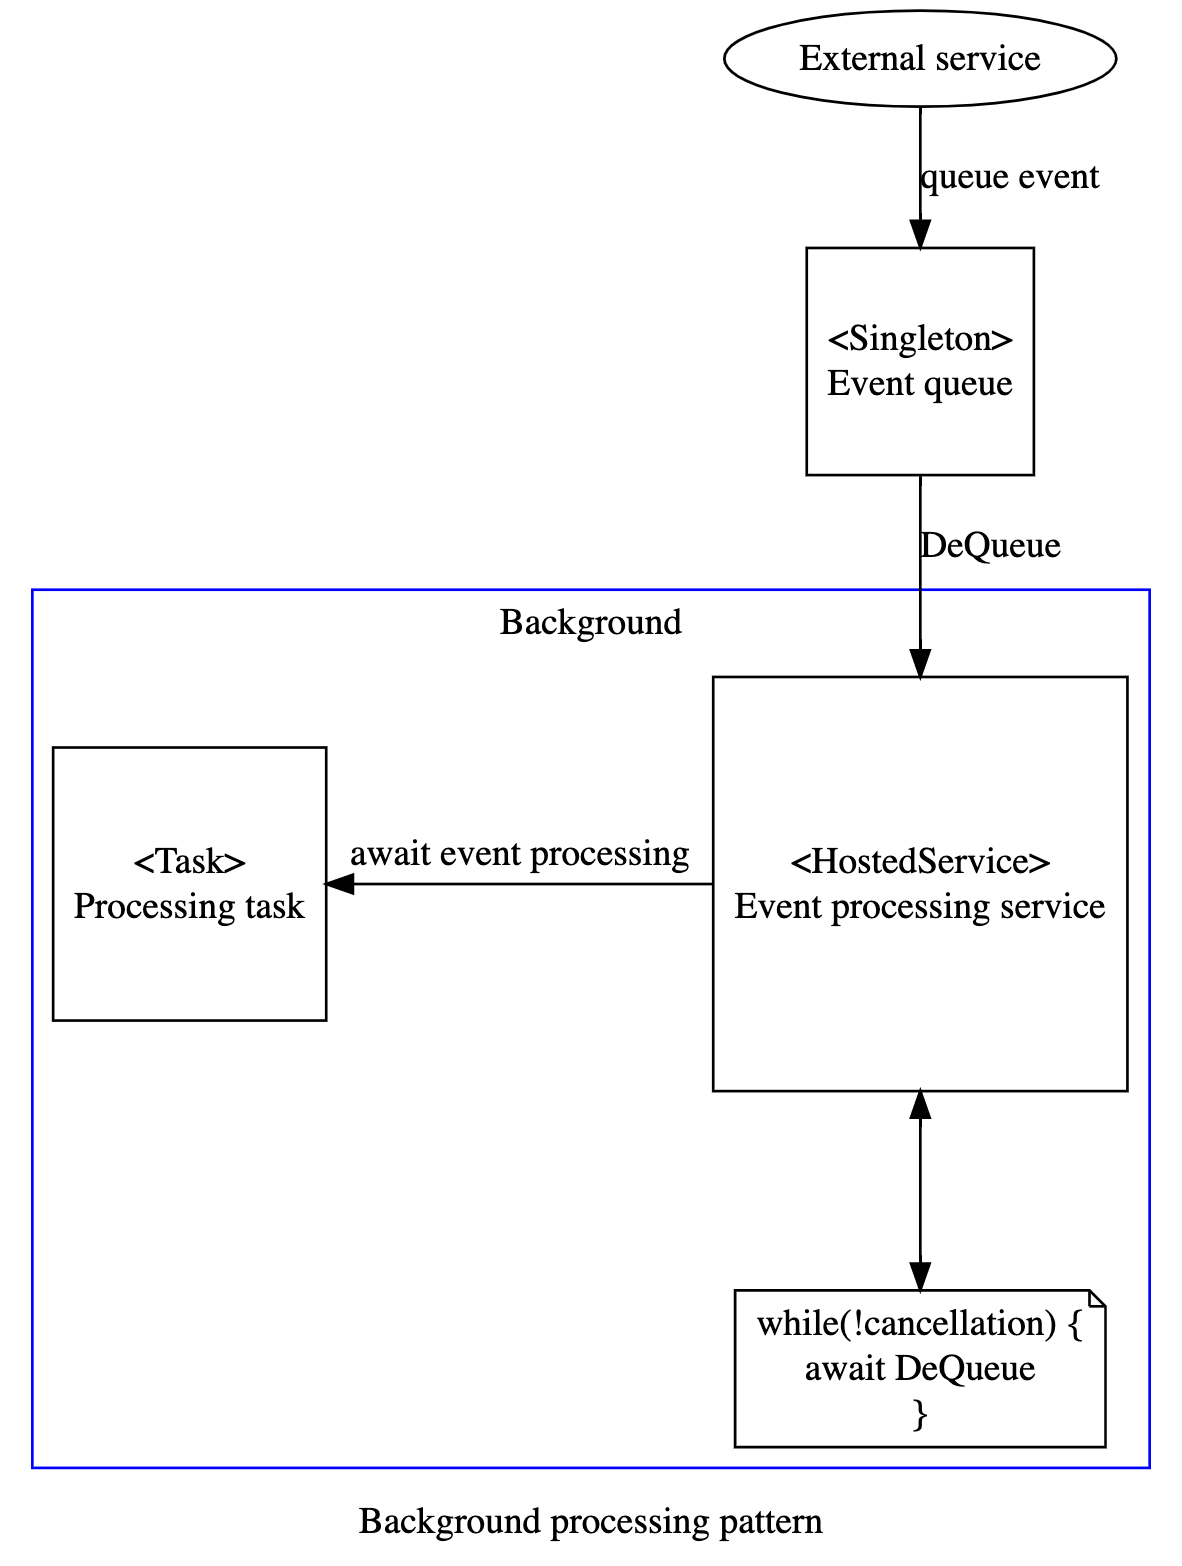
\includegraphics[width=\textwidth,height=\textheight,keepaspectratio]{images/patterns/background-processing-pattern}

\subsubsection{Account management}
% TODO issues with transfer and delete account

\subsection{Database}
% TODO ChainSync™

\subsection{Front-end}

\section{Discussion}
\subsection{Limitation}
% TODO limits of the scope (having to reign in the scope of the project at all points)
% TODO limits of the implementation (gas/price aka no money involved at the moment, transfer and delete wallet, de-sync)

\subsection{Blockchain technology}
% TODO Are these NFTs?
% TODO How long will the blockchain?
% TODO Social consensus/ conflict with governments

\section{Evaluation}
\subsection{Process}
% TODO evaluating my development
% TODO was development agile?

\subsection{Product}
% TODO Has all the functional specifications been met
% TODO Has all the non-functional specs been met
% TODO Does the product fit the target users needs
% TODO Does the product fulfil

\section{Future development}

\begin{description}
	\item[Royalty payments]
	\item[External verification]
	\item[Analytics]
\end{description}

\section{Conclusion}


\bibliographystyle{plain}
\bibliography{sources.bib}

\end{document}
